% !TEX root = main.tex

\section{谓词逻辑}
谓词逻辑(predicate)或被称为一阶逻辑,提供了更强的语言表达能力。

\subsection{形式语言}
\begin{definition}[项(item)]
项的定义如下:
\begin{itemize}
	\item 每一个变量都是项
	\item 若$c\in\mathcal{F}$是一个空函数,则$c$是项(常数)
	\item 若$t_1,t_2,\ldots,t_n$都是项,且$f\in\mathcal{F}$有$n>0$个元(arity),则$f(t_1,t_2,\ldots,t_n)$是一个项
\end{itemize}
用BNF写即
\[t::=x\mid c\mid f(t_1,t_2,\ldots,t_n)\]
\end{definition}
\begin{definition}[公式(formula)]
BNF定义如下
\[\phi::=P(t_1,t_2,\ldots,t_n)\mid
(\lnot\phi)\mid
(\phi\land\psi)\mid
(\phi\lor\psi)\mid
(\phi\to\psi)\mid
(\forall x\phi)\mid
(\exists x\phi)\]
运算符优先级如下
\begin{itemize}
	\item $\lnot,\forall,\exists$
	\item $\lor,\land$
	\item $\to$
\end{itemize}
\end{definition}
\begin{definition}[自由(free)/约束(bound)变量]
语法树叶结点往上不会经过$\forall x$或$\exists x$结点,则为自由变量。
\begin{figure}[H]
\centering
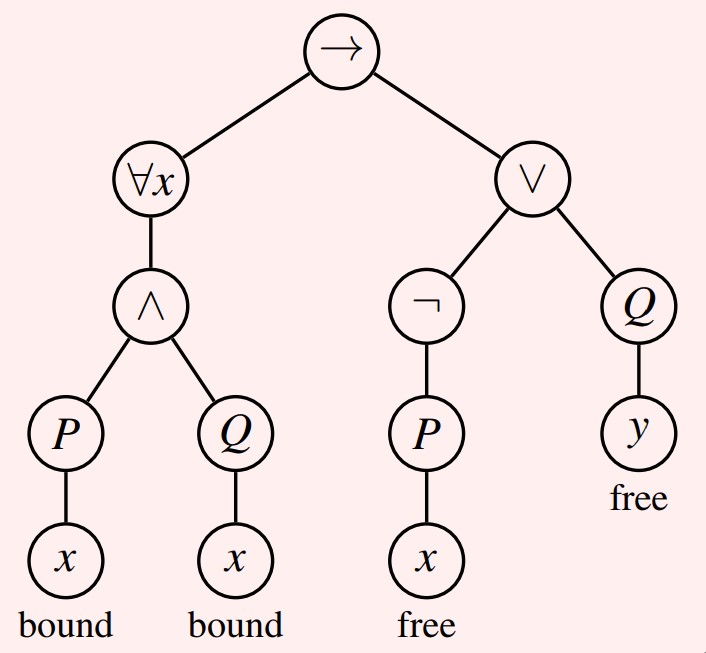
\includegraphics[width=0.4\linewidth]{fig/free_bound_var.jpg}
\end{figure}
\end{definition}
\begin{definition}[替代(substituion)]
给定变量$x$、项$t$和公式$\phi$,定义$\phi[t/x]$为将$\phi$中所有自由$x$用$t$代替
\end{definition}

\subsection{证明论}
\begin{itemize}
	\item equality ($=i$)
	\[\frac{}{t=t}=i\]
	\item substitution ($=e$)
	\[\frac{t_1=t_2\qquad \phi[t_1/x]}{\phi[t_2/x]}=e\]
	\item for-eliminating ($\forall x\quad e$)
	\[\frac{\forall x\phi}{\phi[t/x]}\forall x\quad e\]
	\item for-introduction ($\forall x\quad i$)
	\[\frac{\fbox{\begin{tabular}{c}$x_0$(fresh/dummy var)\\$\vdots$\\$\phi[x_0/x]$\end{tabular}}}{\forall x\phi}\forall x\quad i\]
	\item exists-introduction ($\exists x\quad i$)
	\[\frac{\phi[t/x]}{\exists x\phi}\exists x\quad i\]
	\item exists-elimination ($\exists e$)
	\[\frac{\exists x\phi\quad \fbox{\begin{tabular}{c}$x_0$\quad $\phi[x_0/x]$\\$\vdots$\\$\chi$\end{tabular}}}{\chi}\exists e\]
\end{itemize}
\begin{example}
证明$\forall x(P(x)\to Q(x)),\forall xP(x)\vdash\forall xQ(x)$
\end{example}
\begin{analysis}
推理过程如下
\begin{center}
\begin{tabular}{lll}
1 & $\forall x(P(x)\to Q(x))$ & premise\\
2 & $\forall xP(x)$ & premise\\
3 & $P(x_0)\to Q(x_0)$ & $\forall x\quad e\quad 1$\\
4 & $P(x_0)$ & $\forall x\quad e\quad 2$\\
5 & $Q(x_0)$ & $\to e\quad 3,4$\\
6 & $\forall xQ(x)$ & $\forall x\quad i\quad 3-5$
\end{tabular}
\end{center}
\end{analysis}
\begin{theorem}[等价性(equivalence)]
令$\phi$和$\psi$都为谓词逻辑的公式,有以下等价性
\[\lnot\forall x\phi\dashv\vdash\exists x\lnot\phi,\qquad\lnot\exists x\phi\dashv\vdash\forall x\lnot\phi\]
\end{theorem}

\subsection{语义}
记$\Gamma$为公式$\phi_1,\ldots,\phi_n$,要证明$\Gamma\vdash\psi$是合法的,则只需从$\Gamma$中提供$\psi$的证明。
而如果要证明$\Gamma$推不出$\psi$,从\textbf{证明论}(proof theory)的角度是困难的。

但从语义(semantics)的角度,只需找到一个模型(model)满足所有$\phi_i$都为真,而$\psi$为假,即可得到$\Gamma$推不出$\psi$;相反地,要证明$\Gamma$推出$\psi$则是困难的,因为对于谓词逻辑来说有无穷多种估值/模型,只有全部验证了才能得知$\Gamma\models\psi$($\psi$被$\Gamma$语义蕴含entail)。

因此证明论和模型论两者都是重要的。

\begin{definition}[模型(model)]
令$\mathcal{F}$为函数符号的集合,$\mathcal{P}$为谓词符号的集合\footnote{函数符号是一个算子,作用在项上并生成一个新的项/实体(object),比如$+$和$\times$;而谓词符号也是一个算子,作用在项上并生成一个谓词/宣称(claim),比如$<$和$>$。}。
关于$(\mathcal{F},\mathcal{P})$的模型$\mathcal{M}$包含以下数据:
\begin{itemize}
	\item 非空集合$A$:具体值的全集
	\item 对于每一空函数符号$f\in\mathcal{F},f^{\mathcal{M}}\in A$
	\item 对于每一$f\in\mathcal{F}$且元$n>0$,具体函数$f^{\mathcal{M}}:A^n\to A$
	\item 对于每一$P\in\mathcal{P}$且元$n>0$,子集$P^\mathcal{M}\subset A^n$
\end{itemize}
也就是说$f$和$P$仅仅是\textbf{抽象的符号},而$f^{\mathcal{M}}$和$P^{\mathcal{M}}$为\textbf{具体的函数/元素}。\\
也可以说模型给出了一个解释(interpretation)。
\end{definition}
\begin{example}
令$\mF\eqdef\{i\}$,$\mP\eqdef\{R,F\}$,其中$i$是一个常数,$F$是一元谓词符号,$R$是二元谓词符号。
一个模型可以是
\[\begin{aligned}
A &\eqdef\{a,b,c\}\\
i^{\mM} &\eqdef a\\
R^{\mM} &\eqdef\{(a,a),(a,b),(a,c),(b,c),(c,c)\}\\
F^{\mM} &\eqdef\{b,c\}
\end{aligned}\]
那么有$\exists yR(i,y)$为真,$\lnot F(i)$为真。
\end{example}

上面给出了模型的定义,并且使得我们可以直接从$(\mathcal{F},\mathcal{P})$中计算出真值,但我们仍需讨论如何处理全称量词$\forall x\phi$及特称量词$\exists x\phi$,需要检查$\phi$是否对于所有模型中的$a$都成立。
尽管我们可以用$\phi[a/x]$表示,但是$\phi[a/x]$并不是一个逻辑公式,因为$a$不是一个项(term)而是模型中的一个元素。

因此需要限定公式是关于一个环境的(relative to an environment)。
\begin{definition}[环境(environment)/查找表(look-up table)]
对于全集$A$具体值的环境是一个函数$l:var\to A$,定义$l[x\mapsto a]$为从$x$映射到$a$的查找表。
\end{definition}

\begin{definition}[满足关系(satisfaction)]
给定$\mathcal{M}(\mF,\mP)$及环境$l$,定义满足关系$\mM\models_l\phi$。
若$\mM\models_l$成立(hold),则称$\phi$在关于环境$l$的模型$\mM$中计算为$T$。
\end{definition}

\begin{example}
令$F\eqdef\{alma\},P\eqdef\{loves\}$,其中$alma$是常数,$loves(\cdot,\cdot)$是谓词符号。
模型$\mM$包含集合
\[A\eqdef\{a,b,c\},alma^\mM\eqdef a,loves^\mM\eqdef\{(a,a),(b,a),(c,a)\}\]
检查模型$\mM$是否满足
\[\text{None of Alma's lovers' lovers love her.}\]
\[\phi:\forall x\forall y(loves(x,alma)\land loves(y,x)\to\lnot loves(y,alma))\]
令$x\mapsto a$及$y\mapsto b$,又$alma^{\mM}\eqdef a$,得到
\[loves(a,a)\land loves(b,a)\to\lnot loves(b,alma)\]
不成立,故$\mM\not\models\phi$
\end{example}

在命题逻辑中,$\phi_1,\ldots,\phi_n\models\psi$\footnote{$\models$代表语义蕴含(semantic entailment)}当且仅当$\phi_1,\ldots,\phi_n$都估值为$T$,同时$\psi$也估值为$T$。

\begin{definition}
令$\Gamma$为谓词逻辑的公式集合,$\psi$为谓词逻辑的公式
\begin{enumerate}
	\item 语义蕴含$\Gamma\models\psi$成立当且仅当对于\textbf{所有}的模型$\mM$和查找表$l$,只要$\forall \phi\in\Gamma:\mM\models_l\phi$成立,$\mM\models_l\psi$也成立
	\item $\psi$是可满足的(satisfiable)当且仅当\textbf{存在}模型$\mM$和环境$l$使得$\mM\models_l\psi$成立
	\item $\psi$是合法的(valid)当且仅当$\mM\models_l\psi$对于\textbf{所有}模型$\mM$和环境$l$都成立
\end{enumerate}
\end{definition}
\begin{example}
考虑以下语义蕴含关系
\[\forall x(P(x)\to Q(x))\models\forall xP(x)\to\forall xQ(x)\]
令$\mM$为满足$\forall x(P(x)\to Q(x))$的模型,需要证明$\mM$也满足$\forall xP(x)\to\forall xQ(x)$
\begin{itemize}
	\item 若不是每个$\mM$中的元素都满足$P$,则前件为假,显然成立
	\item 若每个$\mM$中的元素都满足$P$,则每一元素都满足$Q$,因为$\mM$满足$\forall x(P(x)\to Q(x))$
\end{itemize}
进而$\mM\models\forall xP(x)\to\forall xQ(x)$
\end{example}
\begin{example}
考虑以下语义蕴含关系
\[\forall xP(x)\to\forall xQ(x)\models\forall x(P(x)\to Q(x))\]
令$A\eqdef\{a,b\},P^\mM\eqdef\{a\},Q^\mM\eqdef\{b\}$,则$\mM\models\forall xP(x)\to\forall xQ(x)$,但$\mM\not\models\forall x(P(x)\to Q(x))$
\end{example}

% \subsection{不可判定性}